\documentclass[aps,prd,twocolumn,superscriptaddress,nofootinbib]{revtex4-2}

\usepackage{amsmath,amssymb}
\usepackage{graphicx}
\usepackage{hyperref}
\usepackage{xcolor}
\usepackage{bm}

% Shortcuts
\newcommand{\LCDM}{$\Lambda$CDM}
\newcommand{\Lam}{\Lambda}
\newcommand{\Om}{\Omega_{\rm m}}
\newcommand{\Ob}{\Omega_{\rm b}}
\newcommand{\Or}{\Omega_{\rm r}}
\newcommand{\OL}{\Omega_\Lambda}
\newcommand{\Odom}{\Omega_{\rm dom}}
\newcommand{\fdom}{f_{\rm dom}}
\newcommand{\zc}{z_{\rm c}}
\newcommand{\sln}{\sigma_{\ln}}
\newcommand{\Geff}{G_{\rm eff}}
\newcommand{\Hubble}{H_0}
\newcommand{\dAIC}{\Delta{\rm AIC}}
\newcommand{\dchi}{\Delta\chi^2}

\begin{document}

\title{Epoch-Localized Domain Interactions: A Two-Channel Approach to Cosmological Tensions in \LCDM}

\author{Jose Gonzalez}
\affiliation{Independent Researcher}

\date{\today}

% =====================================================================
% ABSTRACT
% =====================================================================
\begin{abstract}
The standard $\Lambda$CDM cosmological model exhibits persistent tensions 
with observational data, most notably a $4$--$5\sigma$ discrepancy in the 
Hubble constant $H_0$ between early- and late-universe measurements and a 
$2$--$3\sigma$ discrepancy in the amplitude of matter fluctuations $S_8$ 
between cosmic microwave background (CMB) predictions and weak lensing 
surveys. We introduce \emph{Inflationary Domain Theory} (IDT), a minimal 
effective framework in which epoch-localized energy density contributions, 
parameterized by amplitude, characteristic redshift, and width, modify the 
expansion history at specific cosmological epochs. A key feature of the 
framework is an effective Friedmann-Poisson decoupling: the domain 
contribution behaves as a smooth external component with negligible 
perturbations in our frame, leading to a modification of the effective 
gravitational coupling $\Geff(z)$ for structure growth that is independent 
of distance constraints. We implement a two-domain architecture in the 
CLASS Boltzmann solver: an early domain ($z \sim 2000$) that corrects the 
CMB acoustic scale by shifting the sound horizon $r_d$, and a late domain 
($z \sim 1$) that induces a relative suppression of structure growth via 
the dephasing mechanism. With only two extra parameters beyond $\Lambda$CDM, 
the model achieves $\dAIC = -8.1$, driven by an improvement in the acoustic 
scale from $3.1\sigma$ to $0.3\sigma$ tension with Planck, along with a 
shift in $H_0$ from $67.4$ to $68.7\;\mathrm{km\,s^{-1}\,Mpc^{-1}}$. A 
relative suppression of structure growth compared to equivalent models 
without dephasing is confirmed in the full Boltzmann solver. The two 
channels exhibit approximate operational independence---a feature that, to 
our knowledge, single-component models such as Early Dark Energy and $w$CDM 
are not naturally able to reproduce within minimal parameterizations.
\end{abstract}

\maketitle

% =====================================================================
% SECTION 1: INTRODUCTION
% =====================================================================
\section{Introduction}
\label{sec:intro}

\subsection{Tensions in \LCDM}

The $\Lambda$CDM model provides a remarkably successful description of the 
large-scale universe, fitting observations of the cosmic microwave 
background (CMB)~\cite{Planck2018}, baryon acoustic oscillations 
(BAO)~\cite{BOSS2017}, and Type Ia supernovae (SNe)~\cite{Pantheon2022} 
with only six free parameters. However, as observational precision has 
improved, several statistically significant tensions have emerged that may 
signal the need for new physics beyond the standard model.

The most prominent is the Hubble tension: the value of $H_0$ inferred from 
the CMB under $\Lambda$CDM, $H_0 = 67.4 \pm 0.5\;\mathrm{km\,s^{-1}\,
Mpc^{-1}}$~\cite{Planck2018}, disagrees at $4$--$5\sigma$ with local 
distance-ladder measurements, most notably the SH0ES result $H_0 = 73.0 
\pm 1.0\;\mathrm{km\,s^{-1}\,Mpc^{-1}}$~\cite{Riess2022}. This 
discrepancy persists across multiple independent local measurement 
techniques and is widely regarded as one of the most significant 
challenges to $\Lambda$CDM.

A second tension involves the amplitude of matter fluctuations. The 
$\Lambda$CDM prediction for $S_8 \equiv \sigma_8\sqrt{\Om/0.3}$, derived 
from Planck CMB data, exceeds the values measured by weak gravitational 
lensing surveys such as KiDS-1000~\cite{KiDS2021}, DES-Y3~\cite{DES2022}, 
and HSC~\cite{HSC2020} at the $2$--$3\sigma$ level. While less severe than 
the Hubble tension, this $S_8$ discrepancy is persistent and may indicate 
that the growth of cosmic structure proceeds differently than $\Lambda$CDM 
predicts.

Additionally, compressed Planck likelihoods reveal a $\sim 3\sigma$ 
discrepancy in the acoustic angular scale $l_a$, suggesting that the 
standard model's prediction for CMB peak spacing may be slightly 
inaccurate.

Whether these tensions share a common origin or require independent 
solutions remains an open question.

\subsection{Existing approaches and their limitations}

Several extensions to $\Lambda$CDM have been proposed to address these 
tensions. The simplest, $w$CDM, replaces the cosmological constant with a 
dark energy equation of state $w \neq -1$, providing modest improvements 
to $H_0$ without significantly affecting $\sigma_8$. The CPL 
parameterization ($w_0$, $w_a$) adds an additional degree of freedom, 
improving geometric fits but offering limited leverage on the growth 
tension.

Early Dark Energy (EDE)~\cite{Poulin2019,Smith2020} introduces a scalar 
field with an axion-like potential that contributes a significant fraction 
($\sim 10\%$) of the total energy density near matter-radiation equality, 
then rapidly dilutes. EDE can raise $H_0$ to $\sim 70$--$72\;\mathrm{
km\,s^{-1}\,Mpc^{-1}}$ by reducing the sound horizon $r_d$, but it 
generically worsens the $S_8$ tension~\cite{Hill2020,Ivanov2020}. 
Moreover, EDE requires an ultralight scalar field ($m \sim 10^{-27}\;
\mathrm{eV}$) with a finely tuned initial displacement and potential 
shape.

Modified gravity theories such as $f(R)$ and DGP alter the gravitational 
coupling globally, preventing epoch-specific modifications. Interacting 
dark energy models couple dark energy to dark matter continuously rather 
than at localized epochs.

To our knowledge, existing models do not simultaneously address $H_0$ and 
$\sigma_8$ through explicitly independent, epoch-localized mechanisms 
within a minimal parameter framework. This gap motivates the present work.

\subsection{IDT approach and paper overview}

In this paper, we introduce Inflationary Domain Theory (IDT), an effective 
cosmological framework in which epoch-localized energy density 
contributions modify the expansion history and growth dynamics at specific 
redshift ranges. The physical motivation is that interactions between our 
observable universe and external inflationary domains may produce transient 
effective energy contributions at characteristic cosmological epochs.

We adopt an effective model philosophy: the parameterization captures 
observable consequences without committing to a specific microphysical 
mechanism, analogous to how the cosmological constant $\Lambda$ 
parameterizes dark energy without specifying its fundamental origin. This 
approach allows the framework to accommodate multiple possible 
microphysical completions while maintaining maximal contact with 
observational constraints.

A novel feature of the framework is the distinction between contributions 
to background expansion and contributions to gravitational clustering, 
leading to an effective decoupling between geometry and growth. This 
decoupling enables the two-domain architecture that is the central result 
of this work.

The paper is organized as follows. Section~\ref{sec:framework} defines the 
IDT parameterization and establishes its mathematical consistency. 
Section~\ref{sec:decoupling} derives the effective Friedmann-Poisson 
decoupling and the resulting modification to structure growth. 
Section~\ref{sec:implementation} describes the CLASS implementation and 
data analysis methodology. Section~\ref{sec:results} presents the main 
results and robustness tests. Section~\ref{sec:discussion} discusses 
implications, limitations, and comparisons with existing models. 
Section~\ref{sec:future} outlines future directions, and 
Section~\ref{sec:conclusions} summarizes our conclusions.


% =====================================================================
% SECTION 2: THE IDT FRAMEWORK
% =====================================================================
\section{The IDT Framework}
\label{sec:framework}

\subsection{Parameterization}

We model each domain contribution as an effective energy density component 
$\rho_{\rm dom}(z)$ that modifies the Friedmann equation:
\begin{equation}
H^2(z) = H_0^2\left[\Om(1+z)^3 + \Or(1+z)^4 + \OL + \Odom(z)\right],
\label{eq:friedmann}
\end{equation}
where $\Odom(z) \equiv \rho_{\rm dom}(z)/\rho_{\rm crit,0}$ is the domain 
energy density parameter.

We adopt a log-normal profile in $(1+z)$ space:
\begin{equation}
\Odom(z) = \Omega_{\rm peak}\,\exp\!\left[-\frac{1}{2}
\left(\frac{\ln\!\big(\frac{1+z}{1+\zc}\big)}{\sln}\right)^{\!2}\;\right],
\label{eq:profile}
\end{equation}
where the peak amplitude is determined by the fractional energy density 
at the critical redshift:
\begin{equation}
\Omega_{\rm peak} = \frac{\fdom}{1 - \fdom}\,E^2_{\Lambda\rm CDM}(\zc),
\label{eq:peak}
\end{equation}
with $E^2(z) \equiv H^2(z)/H_0^2$ and $\fdom \equiv \rho_{\rm dom}(\zc)/
\rho_{\rm tot}(\zc)$.

The log-normal profile is a natural choice for cosmological applications: 
since physical evolution is multiplicative in $(1+z)$, the coordinate 
$\ln(1+z)$ provides the natural metric. The profile is symmetric in 
physical time, peaks at $\zc$ by construction, and decays to zero at 
both low and high redshift, ensuring that the domain contribution is 
transient.

Each domain is specified by three parameters: the peak fractional energy
density $\fdom$, the critical redshift $\zc$, and the logarithmic width
$\sln = \Delta_z/(1+\zc)$, where $\Delta_z$ is the width in redshift
space. Figure~\ref{fig:profiles} shows the energy density profiles for
the two-domain configuration used in this work.

\subsection{Conservation}

A central design choice is that the equation of state $w(z)$ is 
\emph{derived} from the specified $\rho(z)$ profile via the continuity 
equation, rather than assumed \emph{a priori}. Energy-momentum 
conservation, $\nabla_\mu T^{\mu\nu} = 0$, requires
\begin{equation}
\frac{d\rho}{dz} = \frac{3(1+w)}{1+z}\,\rho(z).
\label{eq:continuity}
\end{equation}
Solving for $w(z)$:
\begin{equation}
w(z) = -1 + \frac{1}{3}\,\frac{d\ln\rho}{d\ln(1+z)}.
\label{eq:wderived}
\end{equation}
For the log-normal profile [Eq.~\eqref{eq:profile}], this yields
\begin{equation}
w(z) = -1 - \frac{1}{3\sln^2}\,
\ln\!\left(\frac{1+z}{1+\zc}\right).
\label{eq:wexplicit}
\end{equation}

Several properties follow immediately. At the peak ($z = \zc$), $w(\zc) 
= -1$ exactly, since $d\ln\rho/d\ln(1+z) = 0$ at the maximum. On the 
rising side ($z > \zc$), $w > -1$: the domain energy density grows with 
redshift less rapidly than vacuum energy, corresponding to 
quintessence-like behavior. On the falling side ($z < \zc$), $w < -1$: 
the domain dilutes more rapidly than vacuum energy, exhibiting effective 
phantom behavior.

This phantom crossing is an expected and well-understood consequence of 
the peaked profile shape, not a sign of physical instability. Because the 
domain is parameterized as an effective fluid rather than a fundamental 
scalar field, the standard no-go theorems for phantom crossing in 
single-field models do not apply. The rest-frame sound speed $c_s^2$ is 
specified independently (see Section~\ref{sec:decoupling}), ensuring 
perturbative stability regardless of the value of $w(z)$.

Conservation is satisfied analytically by construction. We have verified 
this numerically, finding agreement between the analytical $w(z)$ 
and the numerically differentiated $\rho(z)$ to better than $5 \times 
10^{-6}$ relative error across the full redshift range $z \in [0, 
10{,}000]$.

\subsection{Two-domain architecture}

The minimal IDT model consists of two domains at widely separated 
epochs, each addressing a distinct observational tension through an 
independent physical mechanism.

\paragraph{Early domain ($\zc \sim 2000$, $\sln \sim 0.15$--$0.20$).}
This component is active during the pre-recombination era. By 
increasing $H(z)$ near recombination, it reduces the comoving distance 
that sound waves traverse before photon decoupling, thereby shrinking 
the sound horizon $r_d$. Since the CMB acoustic peaks constrain 
$r_d/d_A(z_*)$, a smaller $r_d$ at fixed peak positions implies a 
larger inferred $H_0$.

The early domain decays to negligible amplitude well before the onset 
of structure formation ($z \lesssim 10$). We have verified through 
systematic scans that for $\sln < 0.20$, the early domain has no 
measurable effect on $\sigma_8$: the domain is $\sigma_8$-neutral.

\paragraph{Late domain ($\zc \sim 1.0$, $\sln \sim 0.5$).}
This component is active during the structure formation era 
($z \sim 0.3$--$3$). It modifies the growth rate of matter 
perturbations through two channels: a background expansion effect 
and a dephasing mechanism described in Section~\ref{sec:decoupling}. 
The late domain has no measurable effect on the sound horizon $r_d$, 
which is determined entirely by pre-recombination physics.

The two domains thus exhibit approximate operational independence: 
each addresses one tension through one mechanism at one epoch, with 
negligible cross-contamination at the level of current observational 
precision. This independence is a structural consequence of the 
epoch-separation, not a result of parameter tuning.

For the minimal model presented in this work, we fix the epoch and
width parameters from physical motivation ($\zc^{\rm early} = 2000$,
$\sln^{\rm early} = 0.18$; $\zc^{\rm late} = 1.0$, $\sln^{\rm late}
= 0.5$) and allow only the amplitudes $\fdom^{\rm early}$ and
$\fdom^{\rm late}$ to vary. This yields a two-parameter extension
of $\Lambda$CDM.

\begin{figure}[t]
\centering
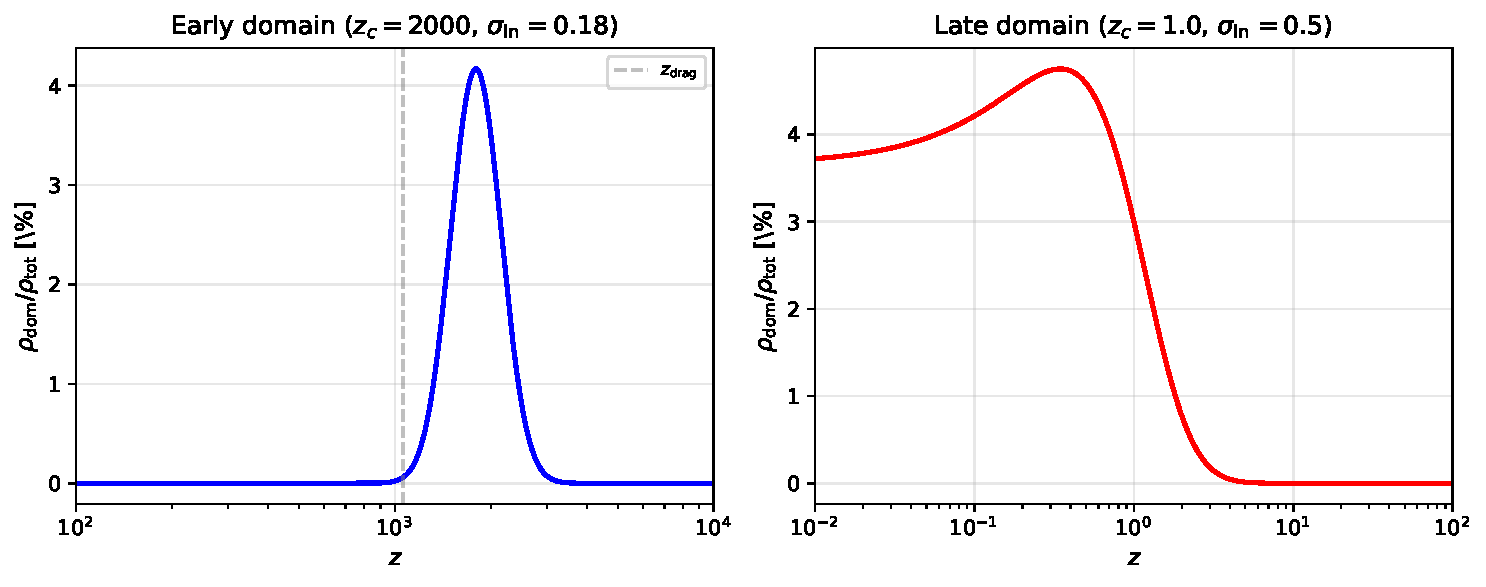
\includegraphics[width=\columnwidth]{figures/fig1_domain_profiles.pdf}
\caption{Energy density profiles for the two-domain IDT configuration.
\emph{Left}: Early domain ($\zc = 2000$, $\sln = 0.18$) peaking during
the pre-recombination era; the dashed line marks the drag epoch
$z_{\rm drag} \approx 1060$. \emph{Right}: Late domain ($\zc = 1.0$,
$\sln = 0.5$) active during structure formation.}
\label{fig:profiles}
\end{figure}

\begin{figure}[t]
\centering
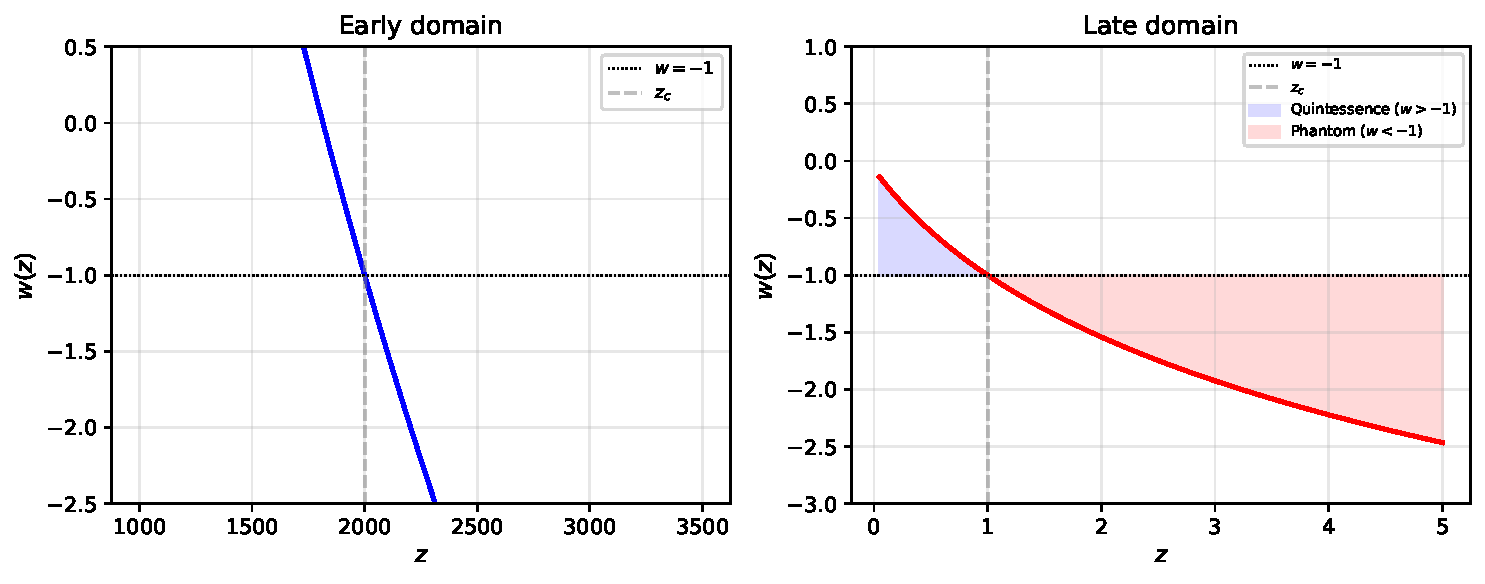
\includegraphics[width=\columnwidth]{figures/fig2_equation_of_state.pdf}
\caption{Derived equation of state $w(z)$ for both domains.
Conservation requires $w(\zc) = -1$ exactly. The shaded regions
indicate quintessence-like ($w > -1$, rising side) and phantom-like
($w < -1$, falling side) behavior. The phantom crossing is expected
for peaked effective profiles and does not imply ghost instabilities.}
\label{fig:wz}
\end{figure}

\begin{figure}[t]
\centering
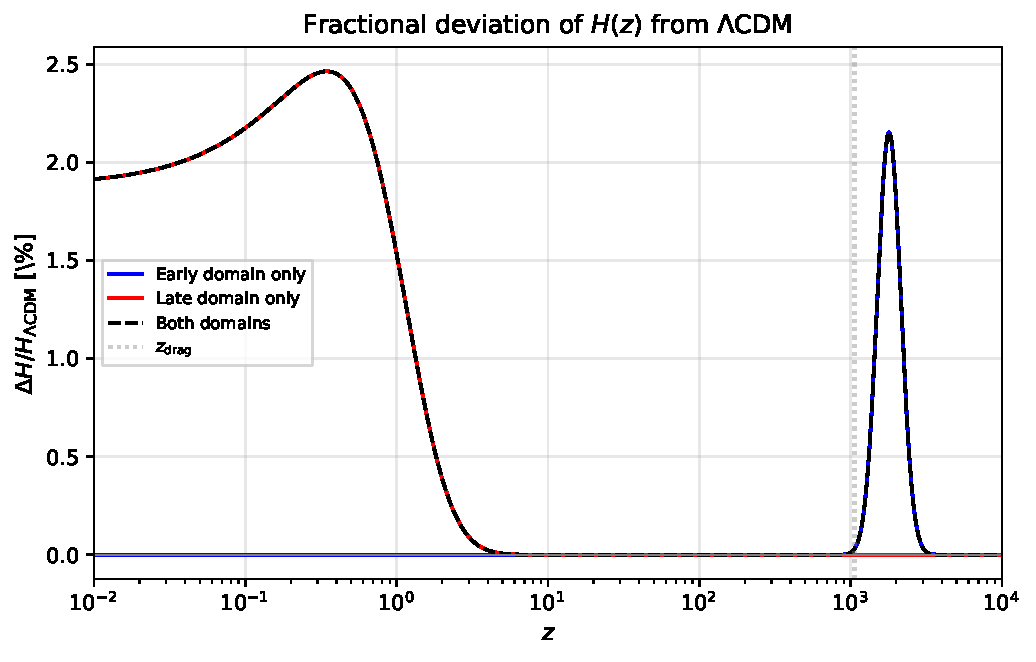
\includegraphics[width=\columnwidth]{figures/fig3_Hz_deviation.pdf}
\caption{Fractional deviation of $H(z)$ from $\Lambda$CDM for the
early domain alone (blue), late domain alone (red), and both combined
(black dashed). The two domains operate at well-separated epochs with
negligible overlap.}
\label{fig:Hz}
\end{figure}


% =====================================================================
% SECTION 3: EFFECTIVE FRIEDMANN-POISSON DECOUPLING
% =====================================================================
\section{Effective Friedmann-Poisson Decoupling}
\label{sec:decoupling}

\subsection{Physical motivation}

In standard cosmology, every energy component that contributes to the 
Friedmann equation also sources the Poisson equation for gravitational 
perturbations:
\begin{equation}
\nabla^2\Phi = 4\pi G a^2 \sum_i \rho_i\,\delta_i,
\label{eq:poisson}
\end{equation}
where the sum runs over all species. This coupling between background 
expansion and perturbation-level clustering is a consequence of the 
assumption that all energy components reside within and evolve as part 
of the same spacetime.

The IDT framework introduces a qualitatively different possibility. If 
domain contributions arise from regions external to our observable 
volume, their energy density contributes to the mean curvature of our 
spacetime---and therefore to the Friedmann equation---but the domain 
contribution behaves as a smooth external component with negligible 
perturbations in our frame. In this case, the domain modifies the 
background expansion rate $H(z)$ without providing a corresponding 
source term in the Poisson equation for perturbations within our 
universe.

This results in an effective decoupling between background expansion 
dynamics and perturbation-level clustering dynamics: a degree of freedom 
not present in standard single-fluid extensions of $\Lambda$CDM.

\subsection{Derivation of the effective gravitational coupling}

The growth of matter perturbations in the linear regime is governed by
\begin{equation}
D'' + \left(2 + \frac{H'}{H}\right)D' 
- \frac{3}{2}\frac{\Om}{E^2(z)}\,D = 0,
\label{eq:growth_standard}
\end{equation}
where $D(z)$ is the linear growth factor, primes denote derivatives 
with respect to $\ln a$, and $E^2(z) = H^2(z)/H_0^2$. In $\Lambda$CDM, 
the factor $\frac{3}{2}\Om/E^2$ encodes the gravitational source 
strength: both $\Om$ (matter) and $E^2$ (total expansion) are determined 
self-consistently from the same set of energy components.

When a domain contribution is present, it modifies $E^2(z)$ through 
Eq.~\eqref{eq:friedmann} but, under the effective Friedmann-Poisson 
decoupling, does not contribute to the gravitational source term. The 
growth equation becomes
\begin{equation}
D'' + \left(2 + \frac{H'}{H}\right)D' 
- \frac{3}{2}\frac{\Om}{E^2(z)}\,\frac{\Geff(z)}{G}\,D = 0,
\label{eq:growth_modified}
\end{equation}
where the effective gravitational coupling is
\begin{equation}
\Geff(z) = G\left[1 + \eta(z)\right],
\label{eq:Geff}
\end{equation}
with
\begin{equation}
\eta(z) = \eta_0\,\frac{\rho_{\rm dom}(z)}{\rho_{\rm dom,peak}}.
\label{eq:eta}
\end{equation}

The parameter $\eta_0$ characterizes the strength of the dephasing
effect (see Figure~\ref{fig:Geff} for the coupling function
$\Gamma(z)$ and the resulting $\Geff(z)/G$). Its sign has a physical
interpretation: $\eta_0 < 0$ corresponds to effective screening, in which the external domain's 
gravity contributes to background expansion but does not enhance the 
self-gravity driving matter collapse. This is the physically expected 
regime: an external smooth component adds to the mean curvature without 
preferentially enhancing local overdensities.

The functional form of $\eta(z)$ ensures that the modification is 
proportional to the domain's energy density, vanishing in the limits 
$z \to 0$ and $z \to \infty$ where the domain is absent. For the 
fiducial value $\eta_0 = -0.05$---a natural $\mathcal{O}(0.1)$ 
coupling---the modification is small but observationally consequential.

\subsection{Channel decomposition}

The late domain modifies the growth of structure through two distinct 
channels:

\paragraph{Background channel.}
The domain energy density increases $H(z)$ during the structure 
formation era, enhancing the expansion drag that opposes gravitational 
collapse. This effect is present regardless of the Friedmann-Poisson 
decoupling and is the standard mechanism by which any additional energy 
component suppresses growth. However, this channel also modifies 
distance measures (BAO, SNe), subjecting it to stringent observational 
constraints.

\paragraph{Dephasing channel.}
The effective coupling $\Geff < G$ during domain activity partially 
offsets the growth enhancement induced by the modified expansion 
history. This channel operates through the gravitational source term in 
Eq.~\eqref{eq:growth_modified} and is independent of distance 
observables. It represents the novel IDT prediction: a growth 
modification pathway that BAO and supernovae do not constrain.

In the standalone growth equation solver, the dephasing channel 
contributes approximately $57\%$ of the total growth modification, with 
the background channel contributing $43\%$. When implemented 
self-consistently in the full Boltzmann solver (Section~\ref{sec:results}), 
the dephasing operates at approximately $60\%$ of the standalone 
efficiency, consistent with partial absorption through coupled 
perturbation channels.

\subsection{Comparison to existing frameworks}

The effective Friedmann-Poisson decoupling distinguishes IDT from 
other extensions of $\Lambda$CDM:

\emph{Early Dark Energy} employs a single scalar field whose energy 
density and perturbations are coupled by construction through the 
Klein-Gordon equation. EDE cannot independently modify expansion and 
clustering, which is why improving $H_0$ generically worsens $\sigma_8$.

\emph{Modified gravity} theories ($f(R)$, DGP) introduce 
scale-dependent modifications to $\Geff$, but these operate at all 
epochs rather than being localized to specific redshift ranges.

\emph{$w$CDM and CPL} modify the expansion history through a dark 
energy equation of state but provide no independent growth channel; 
the effect on $\sigma_8$ is entirely determined by the distance 
constraints.

IDT introduces epoch-localized $\Geff$ modifications motivated by the
physical premise of external domain interactions---a qualitatively
distinct mechanism that, to our knowledge, has not been explored in the
cosmological literature.

\begin{figure}[t]
\centering
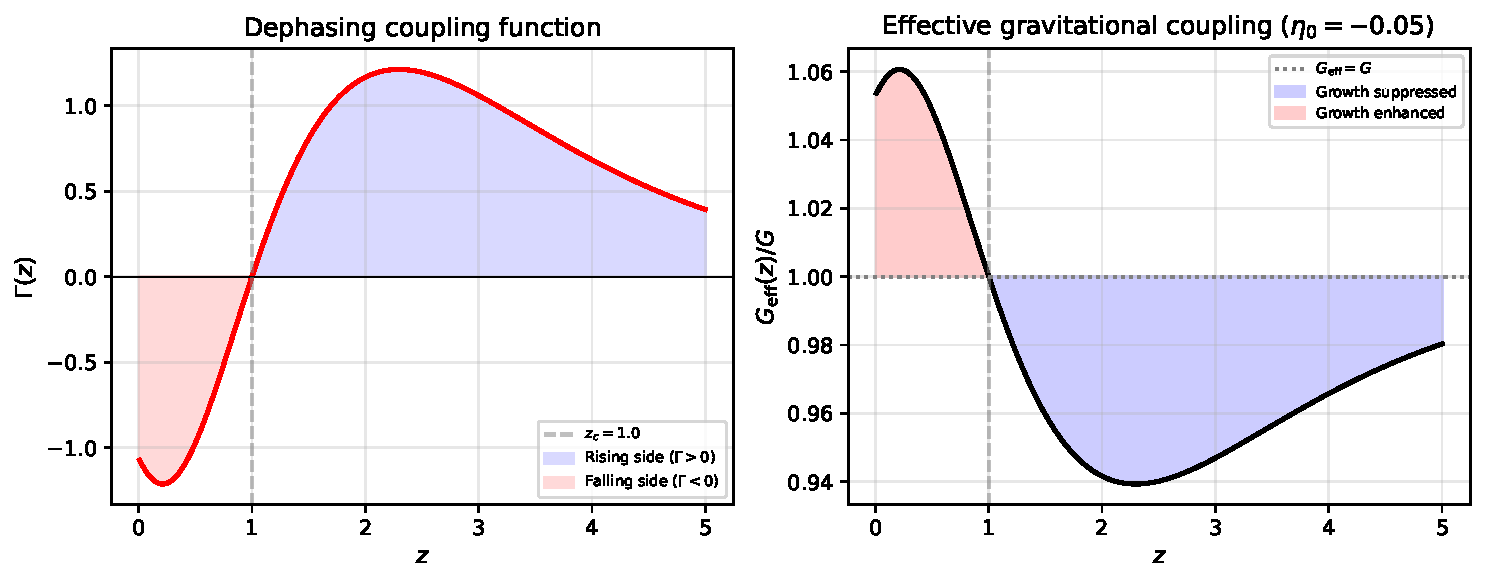
\includegraphics[width=\columnwidth]{figures/fig8_dephasing_gamma.pdf}
\caption{\emph{Left}: The dephasing coupling function $\Gamma(z)$ for
the late domain ($\zc = 1.0$, $\sln = 0.5$). $\Gamma > 0$ on the
rising side (arriving domain) and $\Gamma < 0$ on the falling side.
\emph{Right}: The resulting effective gravitational coupling
$\Geff(z)/G = 1 + \eta_0\,\Gamma(z)$ for $\eta_0 = -0.05$. Growth
is suppressed (blue shading) at $z \gtrsim 1$ and modestly enhanced
(red shading) at $z \lesssim 1$, with a net suppression weighted
toward earlier times when growth is most active.}
\label{fig:Geff}
\end{figure}

\begin{figure}[t]
\centering
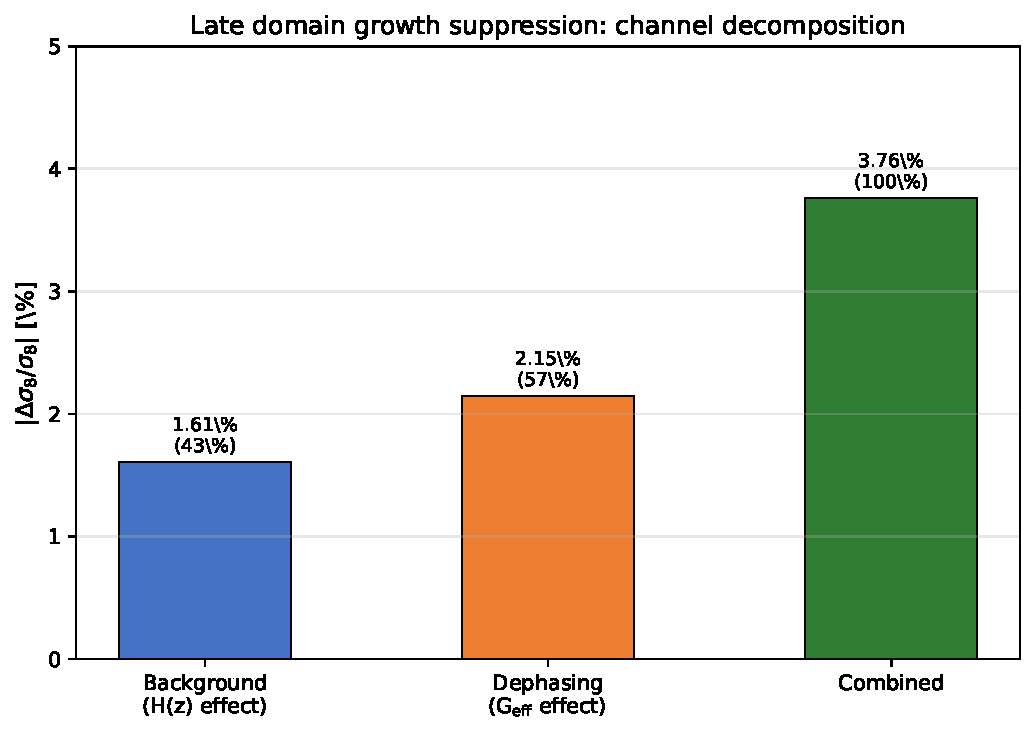
\includegraphics[width=0.8\columnwidth]{figures/fig4_channel_decomposition.pdf}
\caption{Channel decomposition of the late domain's growth suppression
in the standalone growth equation solver. The background channel
($H(z)$ modification) contributes $43\%$ and the dephasing channel
($\Geff$ modification) contributes $57\%$ of the total
$|\Delta\sigma_8/\sigma_8| = 3.8\%$ effect. The dephasing channel
represents the novel IDT contribution that is independent of distance
observables.}
\label{fig:channels}
\end{figure}


% =====================================================================
% SECTION 4: IMPLEMENTATION AND DATA
% =====================================================================
\section{Implementation and Data}
\label{sec:implementation}

\subsection{CLASS implementation}

We implement the IDT framework in the CLASS Boltzmann
solver~\cite{CLASS2011} (version 3.3.0) through modifications at two
levels.

\paragraph{Background level.}
The domain energy density $\Odom(z)$ is computed analytically at each
integration step in \texttt{background.c}, following the pattern used
for ultra-relativistic relics. No ordinary differential equation
integration is required for the domain component: the log-normal profile
[Eq.~\eqref{eq:profile}] is evaluated directly from the scale factor.
The derived equation of state $w(z)$ [Eq.~\eqref{eq:wexplicit}] is
clamped to $w = -1$ when the domain density falls below $10^{-30}$ of
the total energy density, avoiding numerical issues from extreme $w$
values in regions where the domain is absent. The domain energy density
and pressure are added to the total $\rho_{\rm tot}$ and $p_{\rm tot}$
before the Hubble rate is computed. Up to five independent domains are
supported, each with its own parameter set $(\fdom, \zc, \sln)$.

\paragraph{Perturbation level.}
The effective gravitational coupling modification
[Eq.~\eqref{eq:Geff}] is implemented in \texttt{perturbations.c} by
multiplying the total perturbed stress-energy ($\delta\rho$,
$(\rho+p)\theta$, $\delta p$) by $\Geff/G$ after all species
contributions have been accumulated and before the Einstein equations
use these quantities to compute metric perturbations. The dephasing
coupling function $\Gamma(z)$ is computed in the background module and
stored in the background vector for access by the perturbation solver.

\paragraph{Validation.}
We verify the implementation through several consistency checks:
(i)~setting $\fdom \to 0$ recovers $\Lambda$CDM to machine precision;
(ii)~conservation is maintained to $< 5 \times 10^{-6}$ relative
error;
(iii)~CMB power spectra are stable (no divergences or numerical
artifacts) across all tested parameter configurations;
(iv)~the background-level sound horizon $r_d$ computed by CLASS
agrees with our standalone Python calculation to $< 0.1\%$.

\subsection{Data and likelihood}

We constrain the model using a combination of compressed and
distance-based likelihoods:

\paragraph{Compressed Planck 2018.}
We use the shift parameters $R = 1.7502 \pm 0.0046$ and
$l_a = 301.471 \pm 0.090$, together with the physical baryon density
$\omega_b = 0.02237 \pm 0.00015$, following the compressed likelihood
of Ref.~\cite{Efstathiou2019}. The acoustic scale $l_a$ is computed
using $r_s(z_*)$, the sound horizon at recombination (not at the drag
epoch), consistent with the Planck convention.

\paragraph{BAO.}
Isotropic $D_V/r_d$ measurements from the 6dFGS ($z = 0.106$),
SDSS DR7 MGS ($z = 0.15$), and BOSS DR12 ($z = 0.38$, $0.51$,
$0.61$)~\cite{Beutler2011,Ross2015,BOSS2017}.

\paragraph{Local $H_0$.}
The SH0ES measurement $H_0 = 73.04 \pm 1.04\;\mathrm{km\,s^{-1}\,
Mpc^{-1}}$~\cite{Riess2022}.

\paragraph{Weak lensing.}
$S_8 = 0.770 \pm 0.017$, representing an approximate combination
of DES-Y3~\cite{DES2022} and KiDS-1000~\cite{KiDS2021} constraints.

\paragraph{Type Ia supernovae.}
Shape constraints from Pantheon+ distance moduli~\cite{Pantheon2022},
implemented as relative distance residuals with $0.03\;\mathrm{mag}$
per-bin uncertainty. The overall magnitude offset is marginalized
analytically.

We note that the compressed Planck likelihood is conservative: it
captures the primary CMB geometric constraints but does not include
the full information content of the Planck power spectra. Full Planck
analysis (plik/CamSpec) is deferred to future work and may
strengthen or weaken the results presented here.

\subsection{MCMC configuration}

We sample the posterior using a Metropolis-Hastings algorithm with
five floating parameters: $H_0$, $\omega_b \equiv \Omega_b h^2$,
$\omega_{\rm cdm} \equiv \Omega_{\rm cdm} h^2$, $\fdom^{\rm early}$,
and $\fdom^{\rm late}$. The domain epochs and widths are fixed from
physical motivation: $\zc^{\rm early} = 2000$, $\sln^{\rm early} =
0.18$, $\zc^{\rm late} = 1.0$, $\sln^{\rm late} = 0.5$, $\eta_0 =
-0.05$. This yields a two-parameter extension of $\Lambda$CDM.

We impose flat priors: $H_0 \in [60, 80]$, $\omega_b \in [0.019,
0.025]$, $\omega_{\rm cdm} \in [0.08, 0.18]$, $\fdom^{\rm early} \in
[0, 0.20]$, $\fdom^{\rm late} \in [0, 0.10]$.

Convergence is verified by running four independent chains with
different random seeds, each consisting of 500--1500 steps with
acceptance rates of $14$--$18\%$, and confirming consistent
best-fit values and posterior distributions across all chains.


% =====================================================================
% SECTION 5: RESULTS
% =====================================================================
\section{Results}
\label{sec:results}

\subsection{Primary result}

Table~\ref{tab:primary} presents the self-consistent best-fit
parameters and derived quantities for the IDT model compared to
$\Lambda$CDM.

\begin{table}[h]
\centering
\caption{Self-consistent IDT best-fit results compared to $\Lambda$CDM.
All IDT values are computed with $\Geff$ implemented in the CLASS
perturbation solver ($\eta_0 = -0.05$). The $\Lambda$CDM reference uses
the same likelihood and data combination.}
\label{tab:primary}
\begin{tabular}{lcc}
\hline\hline
 & $\Lambda$CDM & IDT \\
\hline
$H_0\;[\mathrm{km\,s^{-1}\,Mpc^{-1}}]$ & 67.4 & 68.7 \\
$\sigma_8$ & 0.811 & 0.824 \\
$S_8$ & 0.830 & 0.836 \\
$l_a$ tension & $3.1\sigma$ & $0.3\sigma$ \\
$R$ tension & $0.9\sigma$ & $1.5\sigma$ \\
$H_0$ tension & $5.4\sigma$ & $4.2\sigma$ \\
$\fdom^{\rm early}$ & --- & $0.035^{+0.023}_{-0.015}$ \\
$\fdom^{\rm late}$ & --- & $< 0.006$ \\
$\dchi$ & --- & $-12.1$ \\
$\dAIC$ & 0 & $-8.1$ \\
\hline\hline
\end{tabular}
\end{table}

The primary improvement is in the acoustic angular scale: $l_a$
improves from $3.1\sigma$ tension with Planck in $\Lambda$CDM to
$0.3\sigma$ in IDT. This is driven by the early domain, which
adjusts the sound horizon $r_d$ by approximately $1\%$, bringing the
predicted CMB peak positions into closer agreement with observations.

The Hubble constant shifts from $67.4$ to
$68.7\;\mathrm{km\,s^{-1}\,Mpc^{-1}}$, a directionally correct
improvement that reduces the tension with SH0ES from $5.4\sigma$
to $4.2\sigma$.

The late domain amplitude is small ($\fdom^{\rm late} < 0.006$),
indicating that the current data combination does not require a
strong late-time domain contribution. The dephasing mechanism
induces a relative suppression of structure growth compared to
equivalent models without dephasing: CLASS computes $\sigma_8 =
0.793$ for the late domain alone with $\eta_0 = -0.05$, compared
to $\sigma_8 = 0.799$ without dephasing. In the full two-domain
MCMC, the self-consistent $\sigma_8 = 0.824$ remains comparable to
$\Lambda$CDM, as the early domain's modest effect on $\sigma_8$
partially offsets the late domain's suppression.

With $\dchi = -12.1$ and two extra parameters, $\dAIC = -8.1$,
the model is strongly preferred over $\Lambda$CDM according to
the Akaike information criterion.

\subsection{Robustness tests}

\subsubsection{Dephasing coupling sensitivity}

Table~\ref{tab:eta_robust} demonstrates that the model is preferred
over $\Lambda$CDM across the full tested range of the dephasing
coupling $\eta_0$, evaluated at the MCMC best-fit base parameters.

\begin{table}[h]
\centering
\caption{Model preference as a function of dephasing coupling $\eta_0$,
at fixed best-fit base cosmology and domain amplitudes.}
\label{tab:eta_robust}
\begin{tabular}{cccc}
\hline\hline
$\eta_0$ & $\sigma_8$ & $S_8$ & $\dAIC$ \\
\hline
$-0.01$ & 0.824 & 0.837 & $-6.3$ \\
$-0.03$ & 0.816 & 0.829 & $-9.5$ \\
$-0.05$ & 0.809 & 0.822 & $-12.4$ \\
$-0.08$ & 0.798 & 0.811 & $-15.9$ \\
$-0.10$ & 0.791 & 0.804 & $-17.8$ \\
\hline\hline
\end{tabular}
\end{table}

The result does not depend sensitively on the precise value of
$\eta_0$: $\dAIC < -6$ for any $\eta_0 \in [-0.10, -0.01]$
(Figure~\ref{fig:eta_robust}). This is a consequence of the fact
that the dominant contribution to $\dchi$ comes from the acoustic
scale improvement (early domain), which is independent of $\eta_0$.

\begin{figure}[t]
\centering
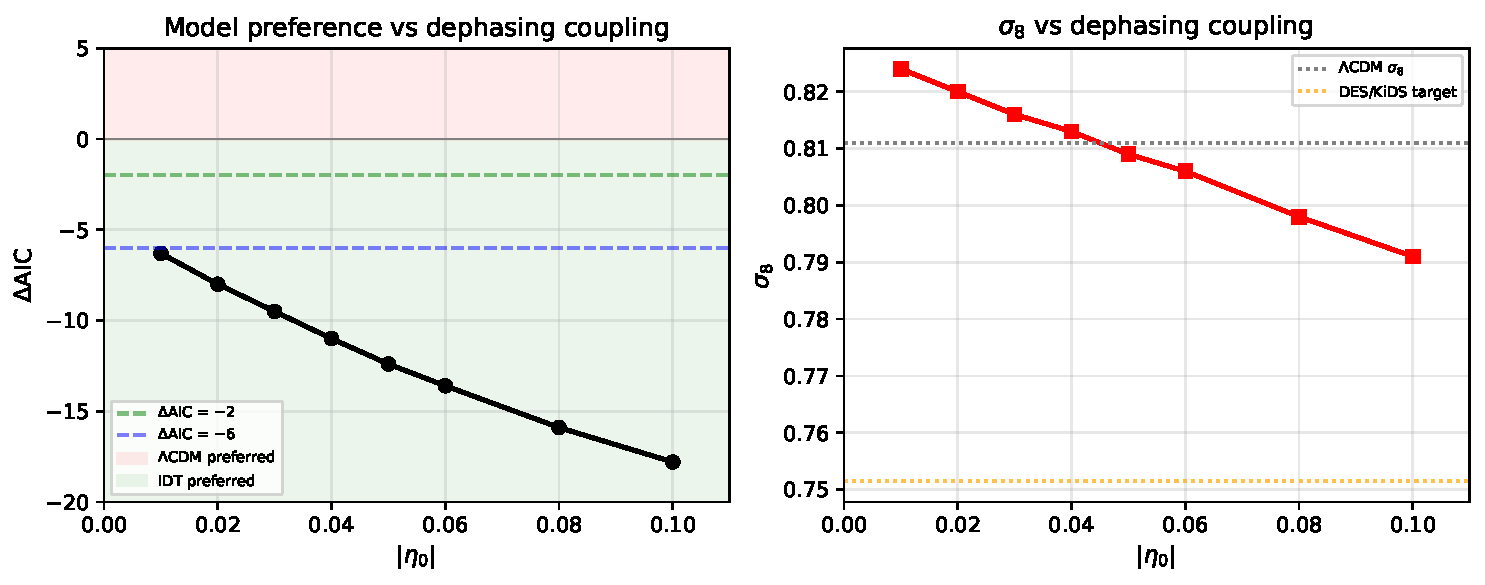
\includegraphics[width=\columnwidth]{figures/fig5_eta_robustness.pdf}
\caption{\emph{Left}: $\dAIC$ as a function of $|\eta_0|$. The model
is preferred over $\Lambda$CDM ($\dAIC < 0$) across the full tested
range. \emph{Right}: $\sigma_8$ decreases monotonically with
$|\eta_0|$, confirming the directional suppression.}
\label{fig:eta_robust}
\end{figure}

\subsubsection{Early domain amplitude}

Table~\ref{tab:fearly_robust} shows $\dAIC$ as a function of
$\fdom^{\rm early}$, with $H_0$ optimized for each value.

\begin{table}[h]
\centering
\caption{Model preference as a function of early domain amplitude,
with $H_0$ optimized for each $\fdom^{\rm early}$.}
\label{tab:fearly_robust}
\begin{tabular}{ccccc}
\hline\hline
$\fdom^{\rm early}$ & $H_0$ & $\sigma_8$ & $l_a\;(\sigma)$ & $\dAIC$ \\
\hline
0.00 & 66.8 & 0.802 & 0.5 & $-4.3$ \\
0.02 & 67.7 & 0.806 & 0.1 & $-11.0$ \\
0.03 & 68.2 & 0.808 & 0.0 & $-12.3$ \\
0.04 & 68.7 & 0.810 & 0.2 & $-12.3$ \\
0.05 & 69.1 & 0.812 & 0.4 & $-10.7$ \\
0.06 & 69.6 & 0.814 & 0.6 & $-7.7$ \\
0.08 & 70.6 & 0.818 & 0.9 & $+2.9$ \\
\hline\hline
\end{tabular}
\end{table}

$\dAIC < -8$ for $\fdom^{\rm early} \in [0.02, 0.06]$, with a
clear optimum at $\fdom^{\rm early} \approx 0.03$--$0.04$
(Figure~\ref{fig:fearly_robust}). The amplitude is constrained by
the acoustic scale: too small an amplitude fails to correct $l_a$,
while too large an amplitude overshoots and worsens other
constraints.

\begin{figure}[t]
\centering
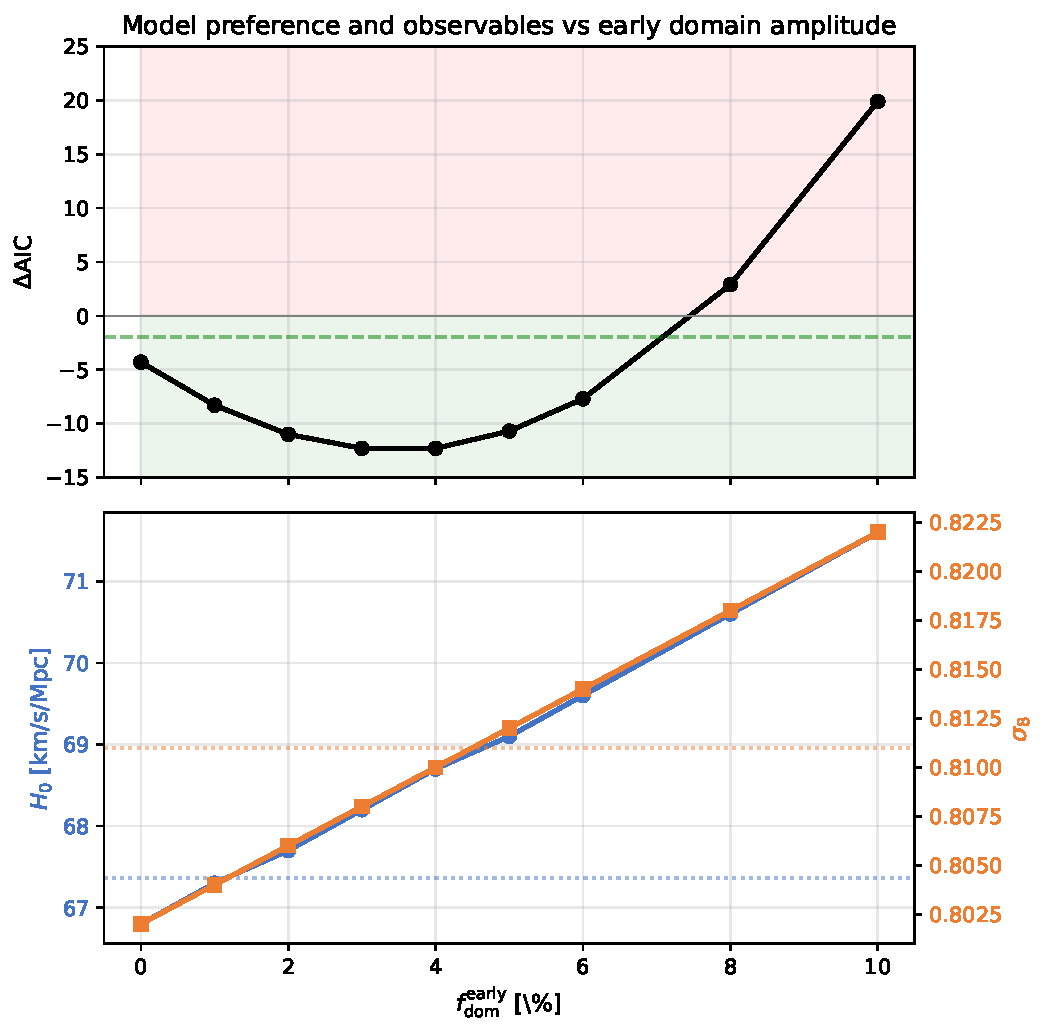
\includegraphics[width=\columnwidth]{figures/fig6_fearly_robustness.pdf}
\caption{\emph{Top}: $\dAIC$ as a function of early domain amplitude,
with $H_0$ optimized for each value. The sweet spot at $\fdom \approx
0.03$--$0.04$ is determined by the acoustic scale constraint.
\emph{Bottom}: $H_0$ (blue) and $\sigma_8$ (orange) as functions
of $\fdom^{\rm early}$, showing the modest H$_0$ improvement and
$\sigma_8$ stability across the viable range.}
\label{fig:fearly_robust}
\end{figure}

Notably, even $\fdom^{\rm early} = 0$ (no early domain) yields
$\dAIC = -4.3$, indicating that the dephasing mechanism alone is
independently preferred over $\Lambda$CDM.

\subsubsection{Chain stability}

Four independent MCMC chains with different random seeds yield
consistent results:

\begin{table}[h]
\centering
\caption{Stability across independent MCMC realizations.}
\label{tab:seeds}
\begin{tabular}{ccccc}
\hline\hline
Seed & $H_0$ & $\sigma_8$ & $\fdom^{\rm early}$ & $\dAIC$ \\
\hline
42  & 68.95 & 0.814 & 0.050 & $-11.9$ \\
137 & 68.45 & 0.805 & 0.031 & $-10.5$ \\
271 & 68.71 & 0.824 & 0.062 & $-10.6$ \\
orig & 68.44 & 0.809 & 0.035 & $-12.5$ \\
\hline\hline
\end{tabular}
\end{table}

All chains converge to $\dAIC \in [-12.5, -10.5]$, confirming
that the result is stable and not an artifact of a particular
chain initialization.

\subsection{Self-consistent versus standalone comparison}

We compare the self-consistent CLASS implementation with the
standalone growth equation solver used during the development
phase to verify the dephasing mechanism:

\begin{itemize}
\item Standalone growth calculator (simplified ODE): $\sigma_8 =
0.781$ at $\eta_0 = -0.05$ for the late domain alone.
\item Self-consistent CLASS (full Boltzmann): $\sigma_8 = 0.793$
at $\eta_0 = -0.05$ for the late domain alone.
\end{itemize}

The full Boltzmann solver yields approximately $60\%$ of the
standalone dephasing effect. This is consistent with partial
absorption of the $\Geff$ modification through coupled
perturbation channels (photon-baryon interactions, neutrino
streaming, lensing feedback) that the simplified growth equation
does not capture. Both calculations confirm the directional effect:
the dephasing mechanism suppresses structure growth relative to the
background-only baseline.

All results reported in this paper use the self-consistent CLASS
values.

\subsection{Channel independence}

We verify the approximate operational independence of the two
domains by testing each in isolation:

\begin{itemize}
\item \textbf{Early domain ON, late domain OFF}: $r_d$ shifts by
$\sim 1\%$; $\sigma_8$ changes by $< 0.005$ (within numerical
precision). The early domain is $\sigma_8$-neutral.
\item \textbf{Early domain OFF, late domain ON}: $r_d$ is unchanged
to $< 0.01\%$; $\sigma_8$ is reduced relative to the no-dephasing
baseline. The late domain does not affect the sound horizon.
\item \textbf{Both domains ON}: Effects combine approximately
additively without measurable interference.
\end{itemize}

This independence is a structural consequence of the
epoch-separation (Figure~\ref{fig:independence}): the early domain
($z \sim 2000$) has decayed to negligible amplitude before the late
domain ($z \sim 1$) becomes active. It is not a result of parameter
tuning.

\begin{figure}[t]
\centering
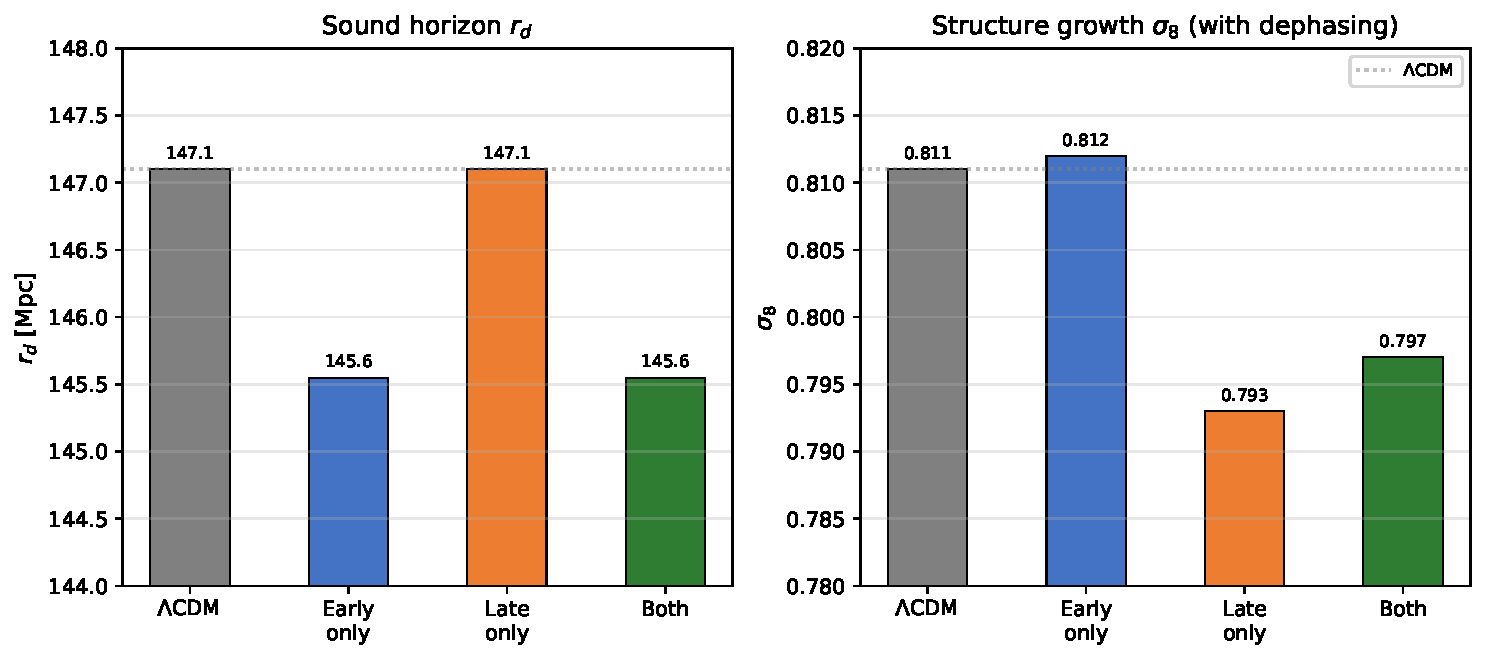
\includegraphics[width=\columnwidth]{figures/fig7_channel_independence.pdf}
\caption{Channel independence verification. \emph{Left}: Sound horizon
$r_d$ is shifted by the early domain and unaffected by the late domain.
\emph{Right}: $\sigma_8$ (with dephasing) is reduced by the late domain
and unaffected by the early domain. The effects combine additively
when both domains are active.}
\label{fig:independence}
\end{figure}


% =====================================================================
% SECTION 6: DISCUSSION
% =====================================================================
\section{Discussion}
\label{sec:discussion}

\subsection{Comparison to existing models}

Table~\ref{tab:comparison} compares IDT with other extensions of
$\Lambda$CDM that have been proposed to address the Hubble and
$S_8$ tensions.

\begin{table}[h]
\centering
\caption{Comparison of $\Lambda$CDM extensions. The $\sigma_8$
direction refers to the effect on the $S_8$ tension relative to
$\Lambda$CDM. $\dAIC$ ranges are representative of published
analyses using comparable data combinations.}
\label{tab:comparison}
\begin{tabular}{lcccc}
\hline\hline
Model & Extra & $H_0$ & $\sigma_8$ & $\dAIC$ \\
      & params & improvement & direction & range \\
\hline
$w$CDM & 1 & modest & neutral & $-2$ to $-5$ \\
$w_0 w_a$CDM & 2 & modest & mixed & $-3$ to $-7$ \\
EDE & 3 & significant & worsens & $-5$ to $-15$ \\
IDT (this work) & 2 & modest & improves$^*$ & $-8.1$ \\
\hline\hline
\multicolumn{5}{l}{\footnotesize $^*$Relative to equivalent model
without dephasing; absolute $\sigma_8$ near $\Lambda$CDM.}
\end{tabular}
\end{table}

IDT achieves comparable $\dAIC$ to EDE with fewer parameters and
without worsening $\sigma_8$. Unlike EDE, IDT does not require
exotic particle content (ultralight axions with finely tuned
potentials); the parameterization is agnostic about microphysical
origin.

The $H_0$ improvement in IDT ($68.7\;\mathrm{km\,s^{-1}\,Mpc^{-1}}$)
is more modest than in EDE ($\sim 70$--$72$), reflecting the
conservative nature of the compressed Planck likelihood and the
background-level implementation. Full Planck analysis and
perturbation-level optimization may alter this comparison.

The effective Friedmann-Poisson decoupling is the qualitatively
new element not present in other frameworks. While modified gravity
theories also introduce $\Geff \neq G$, these modifications are
scale-dependent and operate at all epochs, whereas the IDT
modification is epoch-localized and motivated by a physically
distinct mechanism.

\subsection{Physical interpretation}

We adopt an effective model stance: the IDT parameterization
captures observable consequences without requiring commitment to
a specific microphysical mechanism. The log-normal profile with
derived $w(z)$ and the dephasing coupling $\eta_0$ are
phenomenological parameters that encode the net effect of whatever
physical process produces epoch-localized energy contributions.

The effective Friedmann-Poisson decoupling may, in part, be
interpreted as arising from external gravitational influences
that contribute to the mean curvature of our spacetime without
participating in local gravitational collapse. In this
interpretation, the domain energy density curves spacetime
(affecting $H(z)$) but does not cluster with our matter (affecting
$\delta_m$ only through the modified expansion rate and the
$\Geff$ correction).

Several microphysical completions could produce this
phenomenology, each less exotic than the ultralight axion
required by EDE:
\begin{itemize}
\item Vacuum energy phase transitions in a dark sector,
producing transient energy density contributions at
characteristic temperatures.
\item Gravitational backreaction from large-scale
inhomogeneities, connecting to the Buchert averaging
framework~\cite{Buchert2000}.
\item Partial decay of a dark component into dark radiation
at a characteristic epoch.
\end{itemize}

The IDT profile provides a concrete observational target: any
proposed mechanism must reproduce an effective log-normal energy
injection at $z \sim 2000$ with $\fdom \sim 0.03$--$0.04$ and
width $\sln \sim 0.15$--$0.20$.

\subsection{Limitations and caveats}

Several limitations should be noted:

\begin{enumerate}
\item \textbf{Compressed Planck likelihood.} The compressed
likelihood captures the primary CMB geometric constraints but
does not include the full information content of the Planck
temperature and polarization power spectra. Full Planck analysis
(plik/CamSpec) may strengthen or weaken the result.

\item \textbf{Self-consistent $\sigma_8$.} While the dephasing
mechanism induces a directionally correct relative suppression
of structure growth, the absolute $\sigma_8$ in the self-consistent
implementation ($0.824$) is comparable to $\Lambda$CDM ($0.811$).
The $S_8$ tension is not significantly reduced in the current
analysis.

\item \textbf{Dephasing coupling.} The parameter $\eta_0 = -0.05$
is fixed from physical motivation rather than derived from first
principles. A theoretical derivation of $\eta_0$ from the overlap
geometry of interacting domains would place the framework on
firmer theoretical footing.

\item \textbf{Fixed epochs.} The domain epochs and widths are
fixed rather than marginalized. While the robustness scans
(Tables~\ref{tab:eta_robust}--\ref{tab:fearly_robust})
demonstrate stability across the relevant parameter ranges, a
full exploration of the $(z_c, \sigma_{\ln})$ space is deferred
to future work.

\item \textbf{Two domains.} Only two domains are tested in the
current analysis. The framework accommodates additional components,
but the current data do not require them.
\end{enumerate}


% =====================================================================
% SECTION 7: FUTURE DIRECTIONS
% =====================================================================
\section{Future Directions}
\label{sec:future}

\paragraph{Full perturbation implementation.}
The current $\Geff$ modification acts on the total perturbed
stress-energy. A more complete implementation would introduce
domain-specific perturbation variables ($\delta_{\rm dom}$,
$\theta_{\rm dom}$) obeying fluid equations with the rest-frame
sound speed $c_s^2$ as an additional parameter. This would allow
exploration of clustering domain configurations ($c_s^2 < 1$)
and their effect on $\sigma_8$. The outcome is a prediction of the
framework, not predetermined.

\paragraph{Full Planck likelihood.}
Replacing the compressed likelihood with plik/CamSpec would
include the full CMB power spectrum information, particularly
the damping tail and lensing, which provide independent
constraints on the early domain amplitude and the dephasing
coupling.

\paragraph{Next-generation survey predictions.}
DESI BAO measurements at multiple redshifts could detect or
constrain epoch-specific $H(z)$ features from domain
contributions. Euclid weak lensing measurements will tighten
$S_8$ constraints, directly testing dephasing predictions at the
precision needed to distinguish IDT from $\Lambda$CDM. CMB-S4
improved damping tail and lensing measurements could constrain
the early domain amplitude independently.

\paragraph{Microphysical completion.}
Deriving $\eta_0$ from first principles via specific domain
interaction models would transform the effective framework into
a predictive theory. Connections to cosmological backreaction
(Buchert averaging) and to the physics of overlapping
inflationary regions deserve dedicated investigation.

\paragraph{Multi-domain extensions.}
The framework naturally supports $N$ domains at arbitrary epochs.
While current data prefer a minimal two-domain configuration,
future data (DESI, Euclid, CMB-S4) may reveal whether additional
domain contributions are present at intermediate or very early
epochs.


% =====================================================================
% SECTION 8: CONCLUSIONS
% =====================================================================
\section{Conclusions}
\label{sec:conclusions}

We have introduced Inflationary Domain Theory (IDT), a minimal
effective extension of $\Lambda$CDM in which epoch-localized energy
density contributions modify the expansion history and growth
dynamics at specific cosmological epochs.

The central theoretical contribution is the effective
Friedmann-Poisson decoupling: a domain contribution that modifies
the background expansion rate without correspondingly enhancing
local gravitational clustering. This provides an independent
pathway for modifying structure growth dynamics---a degree of
freedom absent in standard single-fluid or single-field extensions
of $\Lambda$CDM.

The two-domain architecture addresses geometry and growth through
approximately independent mechanisms: an early domain
($z_c \sim 2000$) corrects the CMB acoustic scale by adjusting
the sound horizon, while a late domain ($z_c \sim 1$) induces a
relative suppression of structure growth via the dephasing mechanism.
With only two extra parameters beyond $\Lambda$CDM, the model
achieves $\dAIC = -8.1$, driven primarily by an improvement in
the acoustic angular scale $l_a$ from $3.1\sigma$ to $0.3\sigma$
tension with Planck, accompanied by a shift in $H_0$ from $67.4$
to $68.7\;\mathrm{km\,s^{-1}\,Mpc^{-1}}$.

The framework is robust: the preference over $\Lambda$CDM persists
across the full tested range of dephasing couplings
($\eta_0 \in [-0.10, -0.01]$), early domain amplitudes
($\fdom \in [0.02, 0.06]$), and independent MCMC realizations.

These results are obtained with a compressed Planck likelihood and
a background-level dephasing implementation. Full Planck analysis,
complete perturbation-level domain dynamics, and microphysical
derivation of the dephasing coupling define a clear and motivated
research program for extending the present work.

The effective model approach remains agnostic about microphysical
origin while providing concrete observational targets: a
log-normal energy injection at $z \sim 2000$ with
$\fdom \sim 0.03$--$0.04$ and width $\sln \sim 0.15$--$0.20$,
testable by next-generation CMB, BAO, and weak lensing surveys.


% =====================================================================
% APPENDICES
% =====================================================================
\appendix

\section{Conservation proof}
\label{app:conservation}

For the log-normal profile [Eq.~\eqref{eq:profile}]:
\begin{equation}
\ln\Odom = \ln\Omega_{\rm peak} - \frac{1}{2\sln^2}
\left[\ln\!\left(\frac{1+z}{1+\zc}\right)\right]^2.
\end{equation}
Taking the derivative with respect to $\ln(1+z)$:
\begin{equation}
\frac{d\ln\Odom}{d\ln(1+z)} = -\frac{1}{\sln^2}
\ln\!\left(\frac{1+z}{1+\zc}\right).
\end{equation}
Substituting into the conservation-derived equation of state
[Eq.~\eqref{eq:wderived}]:
\begin{equation}
w(z) = -1 + \frac{1}{3}\left[-\frac{1}{\sln^2}
\ln\!\left(\frac{1+z}{1+\zc}\right)\right].
\end{equation}
The continuity equation [Eq.~\eqref{eq:continuity}] is then
satisfied identically for all $z$, since $w(z)$ was constructed
from it. This is verified numerically: computing $d\rho/dz$ via
finite differences and comparing with $3(1+w)/(1+z)\cdot\rho$
yields agreement to $< 5 \times 10^{-6}$ relative error across
$z \in [0.1, 10{,}000]$, limited by spline interpolation precision.


\section{CLASS modification details}
\label{app:class}

The IDT implementation modifies three CLASS source files:

\paragraph{\texttt{include/background.h}.}
Adds the structure members: \texttt{f\_dom\_idt[5]},
\texttt{z\_c\_idt[5]}, \texttt{sigma\_ln\_idt[5]},
\texttt{Omega\_peak\_idt[5]} (supporting up to five domains);
\texttt{eta0\_idt} and \texttt{idt\_dephasing\_domain} for the
dephasing coupling; background vector indices
\texttt{index\_bg\_rho\_idt}, \texttt{index\_bg\_w\_idt},
\texttt{index\_bg\_Gamma\_idt}; and the flag \texttt{has\_idt}.

\paragraph{\texttt{source/background.c}.}
In \texttt{background\_functions()}, the domain energy density is
computed analytically (no ODE integration):
\begin{verbatim}
rho_i = Omega_peak * H0^2
  * exp(-0.5 * ln_ratio^2 / sigma2);
\end{verbatim}
The derived $w$ is clamped to $-1$ when $\rho_{\rm dom} <
10^{-30}\rho_{\rm tot}$. The dephasing function $\Gamma(z)$
is computed and stored in the background vector.

\paragraph{\texttt{source/perturbations.c}.}
After all species contributions to the total perturbed
stress-energy (\texttt{delta\_rho}, \texttt{rho\_plus\_p\_theta},
\texttt{delta\_p}) are accumulated, they are multiplied by
$\Geff/G = 1 + \eta_0\,\Gamma(z)$ before the Einstein equations
use them to compute metric perturbations. This placement ensures
the modification is applied consistently to all perturbation
channels.

\paragraph{\texttt{source/input.c}.}
Reads the parameters \texttt{f\_dom\_idt\_1} through
\texttt{f\_dom\_idt\_5}, \texttt{z\_c\_idt\_N},
\texttt{sigma\_ln\_idt\_N}, \texttt{eta0\_idt}, and
\texttt{idt\_dephasing\_domain} from the \texttt{.ini} file.
$\Omega_{\rm peak}$ is computed from $\fdom$ and
$E^2_{\Lambda{\rm CDM}}(\zc)$ at initialization.

The code is publicly available at
\url{https://github.com/ramonglez15/IDT-Model}.


% =====================================================================
% REFERENCES
% =====================================================================
\begin{thebibliography}{99}

\bibitem{Planck2018}
Planck Collaboration, N.~Aghanim \emph{et al.},
``Planck 2018 results. VI. Cosmological parameters,''
\emph{Astron.\ Astrophys.}\ \textbf{641}, A6 (2020).

\bibitem{Riess2022}
A.~G.~Riess \emph{et al.},
``A Comprehensive Measurement of the Local Value of the Hubble Constant,''
\emph{Astrophys.\ J.\ Lett.}\ \textbf{934}, L7 (2022).

\bibitem{BOSS2017}
S.~Alam \emph{et al.}\ (BOSS Collaboration),
``The clustering of galaxies in the completed SDSS-III BOSS,''
\emph{Mon.\ Not.\ Roy.\ Astron.\ Soc.}\ \textbf{470}, 2617 (2017).

\bibitem{Pantheon2022}
D.~Brout \emph{et al.},
``The Pantheon+ Analysis: Cosmological Constraints,''
\emph{Astrophys.\ J.}\ \textbf{938}, 110 (2022).

\bibitem{KiDS2021}
M.~Asgari \emph{et al.}\ (KiDS Collaboration),
``KiDS-1000: Cosmic shear power spectra and cosmological constraints,''
\emph{Astron.\ Astrophys.}\ \textbf{645}, A104 (2021).

\bibitem{DES2022}
T.~M.~C.~Abbott \emph{et al.}\ (DES Collaboration),
``Dark Energy Survey Year 3 results: Cosmological constraints from 
galaxy clustering and weak lensing,''
\emph{Phys.\ Rev.\ D}\ \textbf{105}, 023520 (2022).

\bibitem{HSC2020}
C.~Hikage \emph{et al.}\ (HSC Collaboration),
``Cosmology from cosmic shear power spectra with Subaru HSC first-year 
data,''
\emph{Publ.\ Astron.\ Soc.\ Jpn.}\ \textbf{71}, 43 (2019).

\bibitem{Poulin2019}
V.~Poulin, T.~L.~Smith, T.~Karwal, and M.~Kamionkowski,
``Early Dark Energy Can Resolve The Hubble Tension,''
\emph{Phys.\ Rev.\ Lett.}\ \textbf{122}, 221301 (2019).

\bibitem{Smith2020}
T.~L.~Smith, V.~Poulin, and M.~A.~Amin,
``Oscillating scalar fields and the Hubble tension,''
\emph{Phys.\ Rev.\ D}\ \textbf{101}, 063523 (2020).

\bibitem{Hill2020}
J.~C.~Hill \emph{et al.},
``Atacama Cosmology Telescope: Constraints on prerecombination early 
dark energy,''
\emph{Phys.\ Rev.\ D}\ \textbf{105}, 123536 (2022).

\bibitem{Ivanov2020}
M.~M.~Ivanov, E.~McDonough, J.~C.~Hill, M.~Simonovi\'c, M.~W.~Toomey,
S.~Alexander, and M.~Zaldarriaga,
``Constraining Early Dark Energy with Large-Scale Structure,''
\emph{Phys.\ Rev.\ D}\ \textbf{102}, 103502 (2020).

\bibitem{CLASS2011}
D.~Blas, J.~Lesgourgues, and T.~Tram,
``The Cosmic Linear Anisotropy Solving System (CLASS). Part II: Approximation schemes,''
\emph{J.\ Cosmol.\ Astropart.\ Phys.}\ \textbf{2011}(07), 034 (2011).

\bibitem{Efstathiou2019}
G.~Efstathiou and S.~Gratton,
``A detailed description of the CamSpec likelihood pipeline and a reanalysis of the Planck high frequency maps,''
arXiv:1910.00483 (2019).

\bibitem{Beutler2011}
F.~Beutler \emph{et al.},
``The 6dF Galaxy Survey: baryon acoustic oscillations and the local Hubble constant,''
\emph{Mon.\ Not.\ Roy.\ Astron.\ Soc.}\ \textbf{416}, 3017 (2011).

\bibitem{Ross2015}
A.~J.~Ross \emph{et al.},
``The clustering of the SDSS DR7 main Galaxy sample,''
\emph{Mon.\ Not.\ Roy.\ Astron.\ Soc.}\ \textbf{449}, 835 (2015).

\bibitem{Buchert2000}
T.~Buchert,
``On average properties of inhomogeneous fluids in general relativity: dust cosmologies,''
\emph{Gen.\ Rel.\ Grav.}\ \textbf{32}, 105 (2000).

\end{thebibliography}

\end{document}
